\begin{figure*}[h]
  \centering
  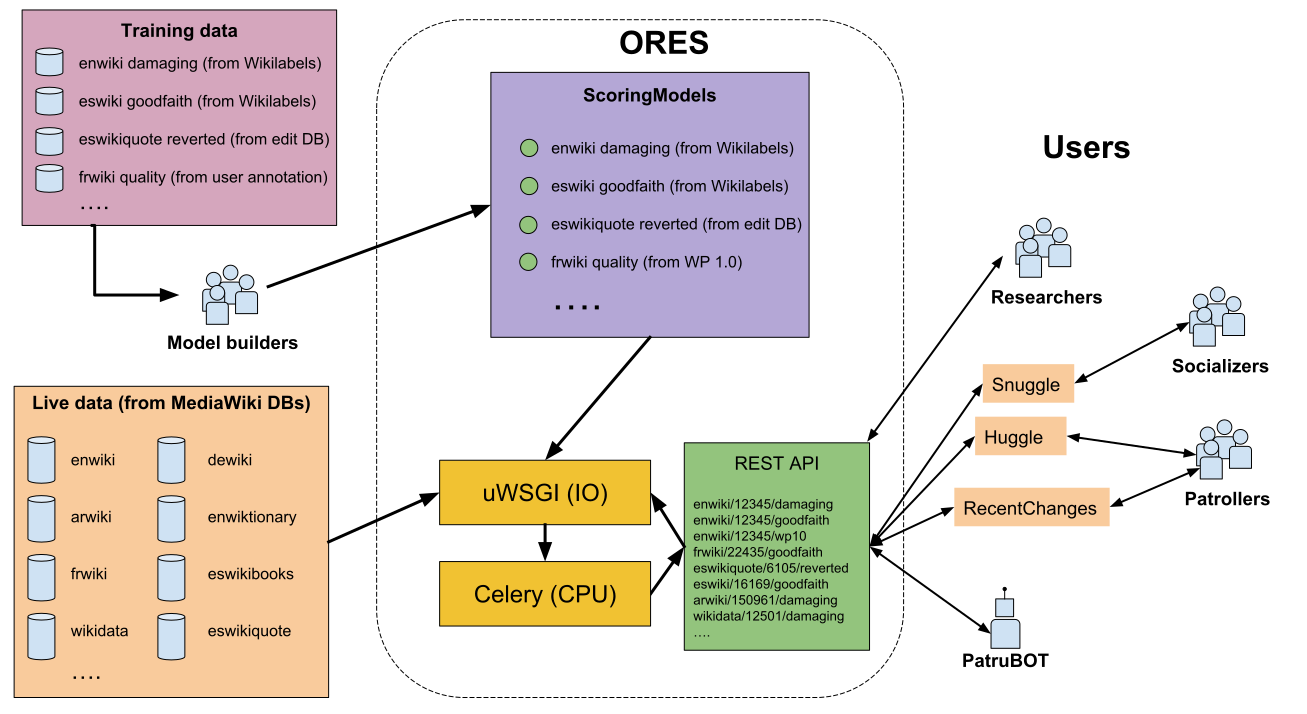
\includegraphics[width=.95\textwidth]{figures/ores_data_user_diagram}
  \caption{ORES conceptual overview.  Model builders design process for training ScoringModels from training data.  ORES hosts ScoringModels and makes them available to researchers and tool developers.}
  \label{fig:ores_data_user}
\end{figure*}

ORES has been iteratively engineered to meet the needs of Wikipedia editors and the tools that support their work.  In this section, we describe how ORES' architecture was built to meet the needs of Wikipedian work processes.

At the core, ORES is a collection of machine classifier models and an API.  These models are designed and engineered by a varied set of model builders (some external researchers and others by our own engineering team) using varied sources of \emph{training data}.  The models that ORES hosts are engineered to support Wikipedian processes related to damage-detection, quality-assessment, and topic-routing, but the system is adaptable to a wide range of other models.

To make these models available for users, ORES implements a simple container service where the ``container,'' referred to as a \emph{ScoringModel}, represents a fully trained and tested prediction model.  All \emph{ScoringModels} contain metadata about when the model was train/tested and code for features extraction.  All predictions take the form of a JSON document.  The ORES service provides access to ScoringModels via a RESTful HTTP interface and serves the predictions (JSON documents) to users.  We chose this service structure because Wikimedian tool developers (our target audience) are familiar with this RESTful API/JSON workflow due to the dominant use of the MediaWiki API among tool developers.  See sections~\ref{sec:appendix} for detailed examples of ORES' outputs and descriptions of how we engineered the system to support Wikipedians' work practices and the tools they use. 
